\documentclass[11pt,letterpaper]{article}
\usepackage{fullpage}
\usepackage{multicol}
\usepackage{amsmath}
\usepackage{amsfonts}
\usepackage{amssymb}
%\usepackage{pstricks, pst-node, pst-plot}

\ifx\pdfoutput\undefined
% we are running LaTeX, not pdflatex
\usepackage{graphicx}
\else
% we are running pdflatex, so convert .eps files to .pdf
\usepackage[pdftex]{graphicx}
\usepackage{epstopdf}
\fi

\newcommand{\ds}{\displaystyle}
\newcommand{\bv}{\mathbf}
\newcommand{\lv}{\langle}
\newcommand{\rv}{\rangle}

\begin{document}
\flushleft
\begin{multicols}{2}


\begin{large}\textbf{Math 116: Extra Credit on Parametric Equations ($\oint 8.2$) \\ 
\begin{flushright} due: Tue 2 Oct 2012 \end{flushright}
}\end{large}

%\textbf{Name:  }\underline{\hspace{35ex}}

\vspace{.5in}

\end{multicols}

\pagestyle{empty}


\flushleft

Find the length of the following parametric curves:
\begin{enumerate}
\item \#17: $x=3+5t,\;y=1+4t$ for $1\leq t\leq 2$.  Explain why your answer is reasonable. 

{\bf Solution:}  Use the arc length formula from page 403.  First, compute the derivatives:
$$x'(t)=5\quad y'(t)=4$$
Then from the formula the arc length is
\begin{align*}\int_a^b\sqrt{x'(t)^2+y'(t)^2}dt &= \int_1^2\sqrt{5^2+4^2}dt \\
&= 2\cdot\sqrt{41}-1\cdot\sqrt{41} \\
&= \sqrt{41} \approx 6.403. 
\end{align*}
To see why this answer makes sense observe we also could have used the Pythagorean Theorem to compute arc length.  The parametrized curve is a line and the bounds $1\leq t\leq 2$ mean we are computing the length from the point $(8,5)$ to $(13,9)$.  The arc length is then given by 
\begin{align*}
\sqrt{\Delta x^2+\Delta y^2} &=\sqrt{(13-8)^2+(9-5)^2} \\
&= \sqrt{5^2+4^2} \\
&=\sqrt{41}.
\end{align*}

\item \#18: $x=\cos{(e^t)},\;y=\sin{(e^t)}$ for $0\leq t\leq 1$.  Explain why your answer is reasonable.

{\bf Solution:} We have
$$x'(t)=-e^t\sin{(e^t)}\quad y'(t)=e^t\cos{(e^t)}$$
and
\begin{align*}
\int_0^1\sqrt{(-e^t\sin{(e^t)})^2+(e^t\cos{(e^t)})^2}\,dt &= \int_0^1\sqrt{e^{2t}(\sin^2{(e^t)}+\cos^2{(e^t)})}\,dt \\
&= \int_0^1e^t\,dt \\
&= e^t|_0^1 \\
&= e-1 \approx 1.718.
\end{align*}
\begin{center}
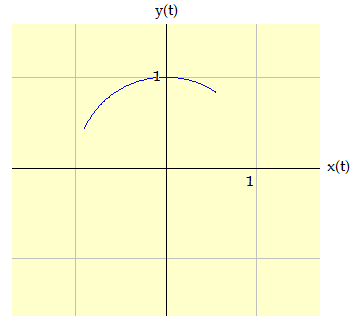
\includegraphics[width=.4\textwidth]{ch8ec.png}
\end{center}
The picture above is the curve we are parametrizing; in this case $x$ and $y$ parametrize the unit circle.  The bounds $0\leq t\leq 1$ give a portion of the circle somewhere between the angles $0$ and $\pi$.  Therefore we would expect the arc length to be a little less than $\pi$, so the answer is reasonable.

\item \#19: $x=\cos{(3t)},\;y=\sin{(5t)}$ for $0\leq t\leq 2\pi$.

{\bf Solution:} This is a straightforward computation, using the arc length formula, then a calculator to evaluate the integral:
\[\int_0^{2\pi}\sqrt{(-3\sin{(3t)})^2+(5\cos{(5t)})^2}\,dt\approx 24.603.\]

\item \#20 $x=\cos^3t,\;y=\sin^3t$, for $0\leq t\leq 2\pi$.

{\bf Solution:} The arc in this case is a closed curve, but if we integrate by a distance of $\frac{\pi}{2}$ at a time and add the results we will get a positive number:
\begin{align*}
\int_0^{2\pi}\sqrt{(-3\cos^2t\sin{t})^2+(3\sin^2t\cos{t})^2}\,dt &= \int_0^{2\pi}\sqrt{9\cos^2t\sin^2t}\,dt \\
&= \int_0^{2\pi}3\cos{t}\sin{t}\,dt \\
&= 6.
\end{align*}

\end{enumerate}

\end{document}


